\documentclass{standalone}
\usepackage{tikz}

\begin{document}\pagestyle{empty}

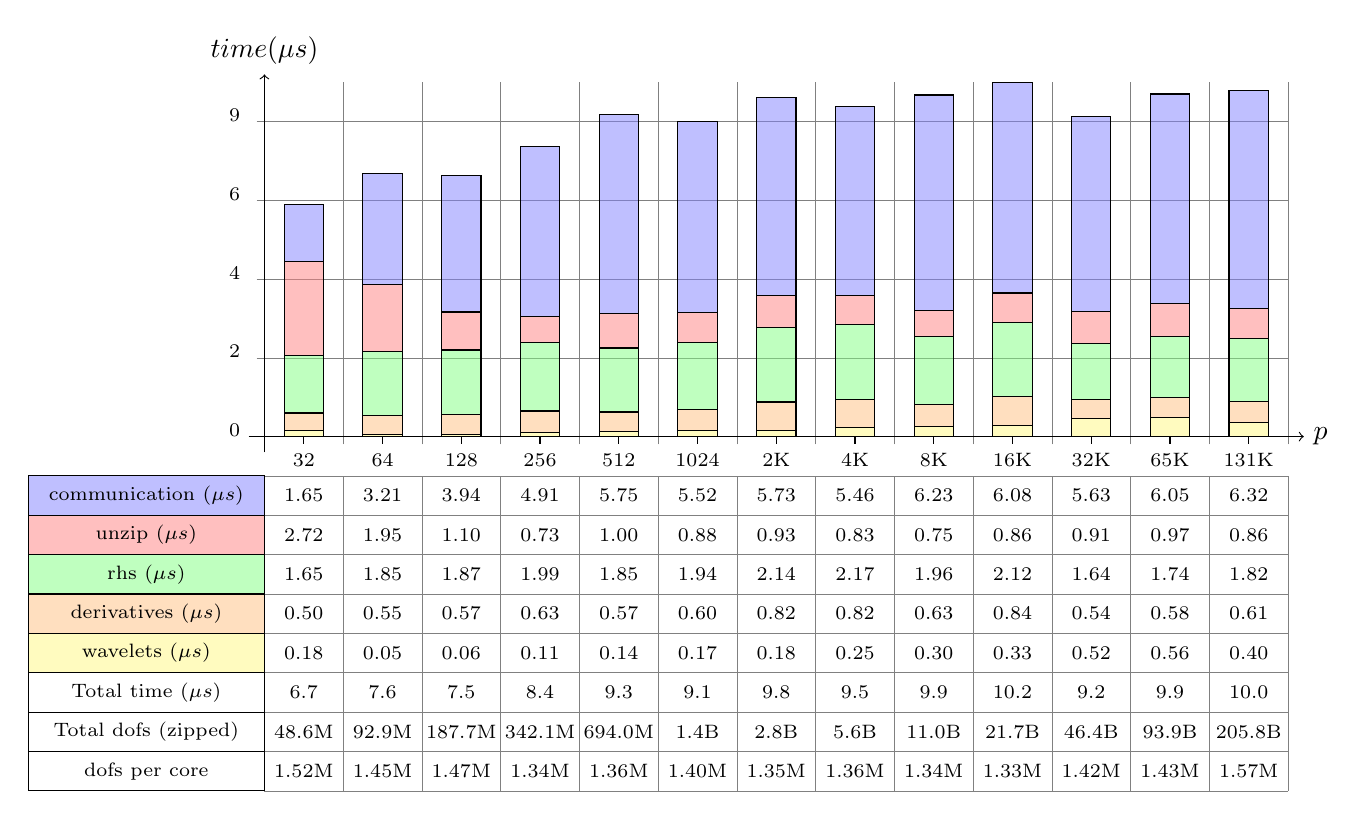
\begin{tikzpicture}

\draw[very thin,color=gray] (-0.1,-0.1) grid (13,4.5);
\draw[->] (-0.2,0) -- (13.2,0) node[right] {$p$};
\draw[->] (0,-0.2) -- (0,4.6) node[above] {$time (\mu s)$};

\foreach \pos/\label in {0.5/32,1.5/64,2.5/128,3.5/256,4.5/512,5.5/1024,6.5/2K,7.5/4K,8.5/8K,9.5/16K,10.5/32K,11.5/65K,12.5/131K}
\draw (\pos,0) -- (\pos,-0.1) (\pos cm,-2.5ex) node [anchor=base,fill=white,inner sep=1pt]  {\scriptsize \label};

\draw[very thin,color=gray, xstep=1, ystep=0.5] (0, -4.5) grid (13,-0.5);
\draw[fill=blue!50, fill opacity=0.5] (-3,-1.0) rectangle +(3,0.5);
\draw (-1.5, -0.75) node {\scriptsize communication $(\mu s)$};

\draw[fill=red!50, fill opacity=0.5] (-3,-1.5) rectangle +(3,0.5);
\draw (-1.5, -1.25) node {\scriptsize unzip $(\mu s)$};

\draw[fill=green!50, fill opacity=0.5] (-3,-2.0) rectangle +(3,0.5);
\draw (-1.5, -1.75) node {\scriptsize rhs $(\mu s)$};

\draw[fill=orange!50, fill opacity=0.5] (-3,-2.5) rectangle +(3,0.5);
\draw (-1.5, -2.25) node {\scriptsize derivatives $(\mu s)$};

\draw[fill=yellow!50, fill opacity=0.5] (-3,-3.0) rectangle +(3,0.5);
\draw (-1.5, -2.75) node {\scriptsize wavelets $(\mu s)$};

\draw (-3,-3.5) rectangle +(3,0.5);
\draw (-1.5, -3.25) node {\scriptsize Total time $(\mu s)$};

\draw (-3,-4.0) rectangle +(3,0.5);
\draw (-1.5, -3.75) node {\scriptsize Total dofs (zipped)};

\draw (-3,-4.5) rectangle +(3,0.5);
\draw (-1.5, -4.25) node {\scriptsize dofs per core};

\draw (-2.5ex, 0 cm) node [anchor=base,fill=white,inner sep=1pt] {\scriptsize 0};

\draw (-2.5ex, 1 cm) node [anchor=base,fill=white,inner sep=1pt] {\scriptsize 2};

\draw (-2.5ex, 2 cm) node [anchor=base,fill=white,inner sep=1pt] {\scriptsize 4};

\draw (-2.5ex, 3 cm) node [anchor=base,fill=white,inner sep=1pt] {\scriptsize 6};

\draw (-2.5ex, 4 cm) node [anchor=base,fill=white,inner sep=1pt] {\scriptsize 9};

\newdimen\mypos
\newdimen\myoff

\foreach \pos/\vala/\valb/\valc/\vald/\vale in { 0/1.65/2.72/1.65/0.50/0.18, 1/3.21/1.95/1.85/0.55/0.05, 2/3.94/1.10/1.87/0.57/0.06, 3/4.91/0.73/1.99/0.63/0.11, 4/5.75/1.00/1.85/0.57/0.14, 5/5.52/0.88/1.94/0.60/0.17, 6/5.73/0.93/2.14/0.82/0.18, 7/5.46/0.83/2.17/0.82/0.25, 8/6.23/0.75/1.96/0.63/0.30, 9/6.08/0.86/2.12/0.84/0.33, 10/5.63/0.91/1.64/0.54/0.52, 11/6.05/0.97/1.74/0.58/0.56, 12/6.32/0.86/1.82/0.61/0.40} { 
\mypos=\pos cm
\advance \mypos by 0.5 cm
\draw (\mypos, -0.75 cm) node {\scriptsize \vala};
\draw (\mypos, -1.25 cm) node {\scriptsize \valb};
\draw (\mypos, -1.75 cm) node {\scriptsize \valc};
\draw (\mypos, -2.25 cm) node {\scriptsize \vald};
\draw (\mypos, -2.75 cm) node {\scriptsize \vale};

\myoff=0 cm

\advance \mypos by -0.25 cm
\draw[fill=yellow!50, fill opacity=0.5, yscale=0.439421279116016] (\mypos,\myoff) rectangle +(0.5,\vale);
\advance \myoff by \vale cm
\draw[fill=orange!50, fill opacity=0.5, yscale=0.439421279116016] (\mypos,\myoff) rectangle +(0.5,\vald);
\advance \myoff by \vald cm
\draw[fill=green!50, fill opacity=0.5, yscale=0.439421279116016] (\mypos,\myoff) rectangle +(0.5,\valc);
\advance \myoff by \valc cm
\draw[fill=red!50, fill opacity=0.5, yscale=0.439421279116016] (\mypos,\myoff) rectangle +(0.5,\valb);
\advance \myoff by \valb cm
\draw[fill=blue!50, fill opacity=0.5, yscale=0.439421279116016] (\mypos,\myoff) rectangle +(0.5,\vala);
\advance \myoff by \vala cm

}

\draw (0.5, -3.25) node {\scriptsize 6.7};
\draw (0.5, -3.75) node {\scriptsize 48.6M};
\draw (0.5, -4.25) node {\scriptsize 1.52M};
\draw (1.5, -3.25) node {\scriptsize 7.6};
\draw (1.5, -3.75) node {\scriptsize 92.9M};
\draw (1.5, -4.25) node {\scriptsize 1.45M};
\draw (2.5, -3.25) node {\scriptsize 7.5};
\draw (2.5, -3.75) node {\scriptsize 187.7M};
\draw (2.5, -4.25) node {\scriptsize 1.47M};
\draw (3.5, -3.25) node {\scriptsize 8.4};
\draw (3.5, -3.75) node {\scriptsize 342.1M};
\draw (3.5, -4.25) node {\scriptsize 1.34M};
\draw (4.5, -3.25) node {\scriptsize 9.3};
\draw (4.5, -3.75) node {\scriptsize 694.0M};
\draw (4.5, -4.25) node {\scriptsize 1.36M};
\draw (5.5, -3.25) node {\scriptsize 9.1};
\draw (5.5, -3.75) node {\scriptsize 1.4B};
\draw (5.5, -4.25) node {\scriptsize 1.40M};
\draw (6.5, -3.25) node {\scriptsize 9.8};
\draw (6.5, -3.75) node {\scriptsize 2.8B};
\draw (6.5, -4.25) node {\scriptsize 1.35M};
\draw (7.5, -3.25) node {\scriptsize 9.5};
\draw (7.5, -3.75) node {\scriptsize 5.6B};
\draw (7.5, -4.25) node {\scriptsize 1.36M};
\draw (8.5, -3.25) node {\scriptsize 9.9};
\draw (8.5, -3.75) node {\scriptsize 11.0B};
\draw (8.5, -4.25) node {\scriptsize 1.34M};
\draw (9.5, -3.25) node {\scriptsize 10.2};
\draw (9.5, -3.75) node {\scriptsize 21.7B};
\draw (9.5, -4.25) node {\scriptsize 1.33M};
\draw (10.5, -3.25) node {\scriptsize 9.2};
\draw (10.5, -3.75) node {\scriptsize 46.4B};
\draw (10.5, -4.25) node {\scriptsize 1.42M};
\draw (11.5, -3.25) node {\scriptsize 9.9};
\draw (11.5, -3.75) node {\scriptsize 93.9B};
\draw (11.5, -4.25) node {\scriptsize 1.43M};
\draw (12.5, -3.25) node {\scriptsize 10.0};
\draw (12.5, -3.75) node {\scriptsize 205.8B};
\draw (12.5, -4.25) node {\scriptsize 1.57M};
\end{tikzpicture}
\end{document}
